%!TEX program = xelatex
\documentclass[11pt, a4paper]{scrartcl}
%\documentclass[11pt, a4paper]{article}
\usepackage[utf8]{inputenc}
%\usepackage[a4paper,lmargin={3.5cm},rmargin={3.5cm}, tmargin={2.5cm},bmargin = {2.5cm}]{geometry}
\usepackage{setspace}
\usepackage{indentfirst}
\usepackage{mathtools}
\usepackage{enumitem}
\usepackage{graphicx}
\usepackage{yfonts, amsmath, amssymb}
\usepackage[backend=biber, authordate, ibidtracker=context, natbib]{biblatex-chicago}
\usepackage{titlesec}
\usepackage{color}
\usepackage{tikz}
\usetikzlibrary{fit,positioning}
\usetikzlibrary{arrows}

\onehalfspacing{}
\addbibresource{bib.bib}

\usepackage{fontspec}
\newfontfamily\osfamily{Latin Modern Roman Demi}

\setkomafont{disposition}{\osfamily}

\renewcommand{\i}[1]{\emph{#1}}
\renewcommand{\L}{\mathcal{L}}
\renewcommand{\v}[1]{\vec{\mathrm{#1}}}

\newcommand{\m}[1]{\textswab{#1}}
\newcommand{\given}[1][]{\:#1\vert\:}

\titleformat{\section}[block]{\Large\bfseries\osfamily\filcenter}{}{1em}{}
%\titleformat{\section}{\Large\bfseries\osfamily}{\thesection}{1em}{}
\titleformat{\subsection}[block]{\large\filcenter}{}{1em}{}
%\titleformat{\subsection}{\large\bfseries\osfamily}{\thesubsection}{1em}{}
%\renewcommand{\thesection}{\Roman{section}} 

\title{\osfamily{}Something Something Imprecise}
\author{Class Paper for Central Topics in Philosophy of Science \\ Prof.\ Dr.\ Stephan Hartmann \\ WS 2017/2018, LMU Munich \\ Conrad Friedrich \\ \texttt{conradfriedrich@posteo.net} \\ Word count: 5643}

\begin{document}

\maketitle
\thispagestyle{empty}
%\tableofcontents
\newpage
\section{I}
Modeling the cognitive state and dynamics of scientists or, more generally, epistemic agents to research predominantly normative issues is a central aspect in the philosophy of science and formal epistemology. In particular, it is crucial to tell a coherent and convincing story about reasoning with uncertain and incomplete information. The all-too-pervasive problem of induction reappears here, too. A crowd favorite in much of these fields is the use of a Bayesian framework, which has proven meaningfully relevant, versatile, and successful (cite Hartmann 1 Hartmann2). So much so that it is not improper to speak of something like a Bayesian orthodoxy in the philosophy of science. More precisely, it is very common to assess questions about evidence and uncertain reasoning within the Bayesian framework, implying the use of the mathematical theory of probabilities to capture doxastic states and reasoning processes of epistemic agents.

\subsection{I}
The Bayesian framework is a method or tool to assess a philosophical problem. The framework forces the philosopher to very precisely state her problem in a quantifiable manner, and repays this effort with the deductive capabilities of probability theory. When such a powerful tool becomes orthodoxy, it might be tempting to disregard the substantial assumptions made just to be able to apply the tool. When you've got a hammer, everything looks like a nail. The method should not be implemented for its own sake, of course, and instead be regulated by some sensible desiderata for a successful use of the method. Two particularly relevant desiderata are somewhat self-evident: (i) the lack of complexity of the framework. Bayesianism is comparably simple: The doxastic state of an agent is modeled by a single probability function. If there is a competing framework which do offer little more for the price of massively increased complexity, it'd be prudent to stick to the Bayes, man. And (ii), models created with the framework need to be adequate. That is, there are no glaring relevant features of the problem that is modeled missing, and the model itself does not produce artifacts not present in the problem. We are in rather murky philosophical waters here, but an intuitive understanding is all we need so far. Note that I do not open Pandora's Box and speak about the balancing of the mentioned and other desiderata.

\subsection{II}
Responsible use of the framework requires careful analysis of the applicability of the framework just as much as of the actual application, then. To respect this, it is especially critical to know the limits and weaknesses, and Bayesianism arguably has its fair share.  

As a stout critic of Bayesianism as a universal theory of induction, \cite{Norton2011-NORCTB} makes a number of substantial challenges, some of which are the subject of the present paper. I will focus on those challenges to Bayesianism which \emph{prima facie} require the use a more elaborate model.

STATE MAIN CLAIM

\subsection{III}
Quick summary of what follows
\section{II}

Quick Recap of Bayesianism: 1) Doxastic attitudes best represented by single probability function + axioms 2) some principle of indifference 

\subsection{I}
Following \cite{Joyce2005-JOYHPR} and \cite{sep-imprecise-probabilities}, there is a very significant point to be made about the \emph{weight} evidence has on a doxastic attitude. Consider this stock example: You have a coin of unknown bias. It may be biased to either side to any degree, or be completely fair. You lack any information. Does it land heads on the next toss? The Bayesian prescribes a precise intermediate credence. Now you start tossing the coin a copious amount, with a very balanced record: about half of the tosses were heads. Pretty good evidence for a fair coin, ej? The Bayesian prescribes the same precise intermediate credence as before, completely disregarding the new-found evidence of the myriad of tosses. In short: An obvious, important shift in the evidential situation is not reflected in the Bayesian framework, hence falling short to account for central and important aspects of the doxastic attitude\footnote{Don't forget to mention beforehand somewhere!}. 

\subsection{II}Relatedly, Bayesianism fails to model the potential \emph{ignorance} of an agent towards a given proposition. To call upon Elga's oft-quoted example:
\begin{quote}
A stranger approaches you on the street and starts pulling out objects from a bag. The first three objects he pulls out are a regular-sized tube of toothpaste, a live jellyfish, and a travel-sized tube of toothpaste. To what degree should you believe that the next object he pulls out will be another tube of toothpaste?
(\cite{Elga2010-ELGSPS})
\end{quote}
While Elga eventually argues for a different point, he and \citet{sep-imprecise-probabilities} make quite a convincing case to be sceptic about a single, precise degree of belief as the rational response to this scenario. Suppose you formed such a belief. What would it be based on? The choice of reference class seems to be completely arbitrary, and hence, not befitting of a single rational probability to ascribe. Alternatively, are there living beings in the orbit around Sirius, a (for these purposes) unknown star, as \citet{Shafer1976-SHAAMT} asks? It seems we just don't know. We are ignorant with respect to this proposition, something that cannot be captured with a precise, additive probability function, says \citet{Norton2011-NORCTB}.

\subsection{III}
Many justifications for the applicability of the Bayesian framework are pragmatic in nature and employ the close connection to decision theoretic considerations. Closely coupled to the doxastic attitudes of an agent is her betting behaviour. It is not surprising then, that results from empirical studies of the betting behaviour of actual people do have some bearing on the applicability of models based on the Bayesian framework, as the famous Ellsberg problem suggests (\cite{10.2307/1884324}, \cite{Camerer1992}). There is no room in this paper to reiterate the problem and to deal with the question of how empirical findings bear on normative considerations, but it is worth noting that on the face of it, the aversion to ambiguity or uncertain risks exhibited by subjects presented with the Ellsberg problem poses a challenge to Bayesians by clashing with desiderata (ii) above (adequacy). It also hints at a more general normative intuition: That sometimes, it is rationally permissible to have \emph{incomparable}\footnote{Or sometimes, more fancifully, incommensurable.} confidence levels towards different propositions. What is more probable, that (A) Tokyo will have a severe earthquake on June 1, 2230; or that (B) Norway will have an unusually good fish catch on that day \citep[p.658]{Jaynes2003-JAYPTT}? It seems entirely innocuous to assume that it is just not meaningful to compare the probabilities, given one lacks some background information. Jaynes himself points out that, with enough context provided, there might be causal links to be hypothesized which enable us to compare the probabilities directly. But lacking that information, it seems at least permissible to judge them as incomparable with respect to the level of uncertainty, which the Bayesian framework cannot account for. 
\subsection{III}

Of course, there are ways to respond for the determined Bayesian. (Briefly list them here, need to get on with it!) 
\section{III}

So far, I have presented three substantial challenges to the Bayesian framework applied in the synchronic case: We just look at a given point in time, and evaluate the adequacy of the probabilistic model. I showed that the Bayesian has the means to respond. Still, as an alternative option that a move to imprecise probabilities solves the problems with ease. In this section, I also consider the diachronic case: a learning experience for the agent. While this is one of the cornerstones of the Bayesian framework through conditionalization, the issue presented here is not easily addressed with a single probability distribution, or so I argue. 

Suppose you learn, with certainty, that the probability of an event $E$ happening lies in some interval $[a,b] \subset [0,1]$, but nothing else about $E$. Specifically, you do not learn that each intermediate interval f the same size is equiprobable. This might just be the meteorologist telling you of the Blizzard hitting your home town is more probable than 15\%, but less than 40\%. Since the information you learn directly deals with probabilities, it seems natural to include the content of the learning experience in a probabilistic model and make the information endogenous.  

\begin{figure}[h]
\centering
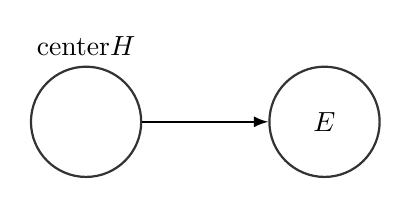
\begin{tikzpicture}
\tikzstyle{main}=[circle, minimum size = 14mm, thick, draw =black!80, node distance = 16mm]
\tikzstyle{connect}=[-latex, thick]
\tikzstyle{box}=[rectangle, draw=black!100]
  \node[main, fill = white!100] (alpha) [label=center$H$] { };
  \node[main] (theta) [right=of alpha,label=center:$E$] { };
  \path (alpha) edge [connect] (theta);
\end{tikzpicture}
\end{figure}

Paragraph about the relevance of the issue: Just vague expert testimony, etc. -> Robust Bayes Analysis, Quantum thingies? 

the dynamic case: learning imprecise information. Missing: Very good scientific example. Also missing: Much of a clue as to how it relates to Robust Bayesian Analysis
\begin{enumerate}[label=\roman{*}]
    \item A simple yet compelling example where the input is imprecise.
    \item Show how naively it isn't darstellable
    \item Show how it isn't darstellable as second order props
    \item Show how it is darstellable as imprecise props 
    \item profit
\end{enumerate}
\section{IV}

Problems: Second order imprecision etc., dilation, 
\section{V}

\begin{singlespacing}
\printbibliography{}
\end{singlespacing}

\end{document}
